\section{Cyberinfrastructure Shell}

% \noindent
% 
\includegraphics[width=90mm]{graphics/cishellLogo.png}

The Cyberinfrastructure Shell (CIShell) \cite{cishell} is an open source, 
software specification for the integration and utilization of datasets, 
algorithms, tools, and computing resources. The Cyberinfrastructure Shell (1) 
supports algorithm writers to write and disseminate their algorithms in their 
favorite programming language while retaining their intellectual rights after 
distribution; (2) data holders to easily disseminate their data for use by 
others; (3) application writers to design applications from custom sets of 
algorithms and datasets that interoperate seamlessly; and finally (4) 
researchers, educators, and practitioners to use existing datasets and 
algorithms to further science.

Algorithm integration support is built in for Java and most other programming 
languages. Being Java based, CIShell runs on almost all platforms. The software 
and specification is released under the Apache 2.0 License.

Subsequently, we describe the bundling, integration, and distribution of 
datasets and algorithms, the deployment of CIShell algorithms as service pools 
or applications, as well as the interlinkage of service pools and applications. 
We then address the issues of automatic data conversion and brandable graphical 
user interfaces (GUIs).

\subsection{Defining Algorithms \& Datasets}

%\begin{wrapfigure}{i}[-2mm]{45mm} 
\begin{center}
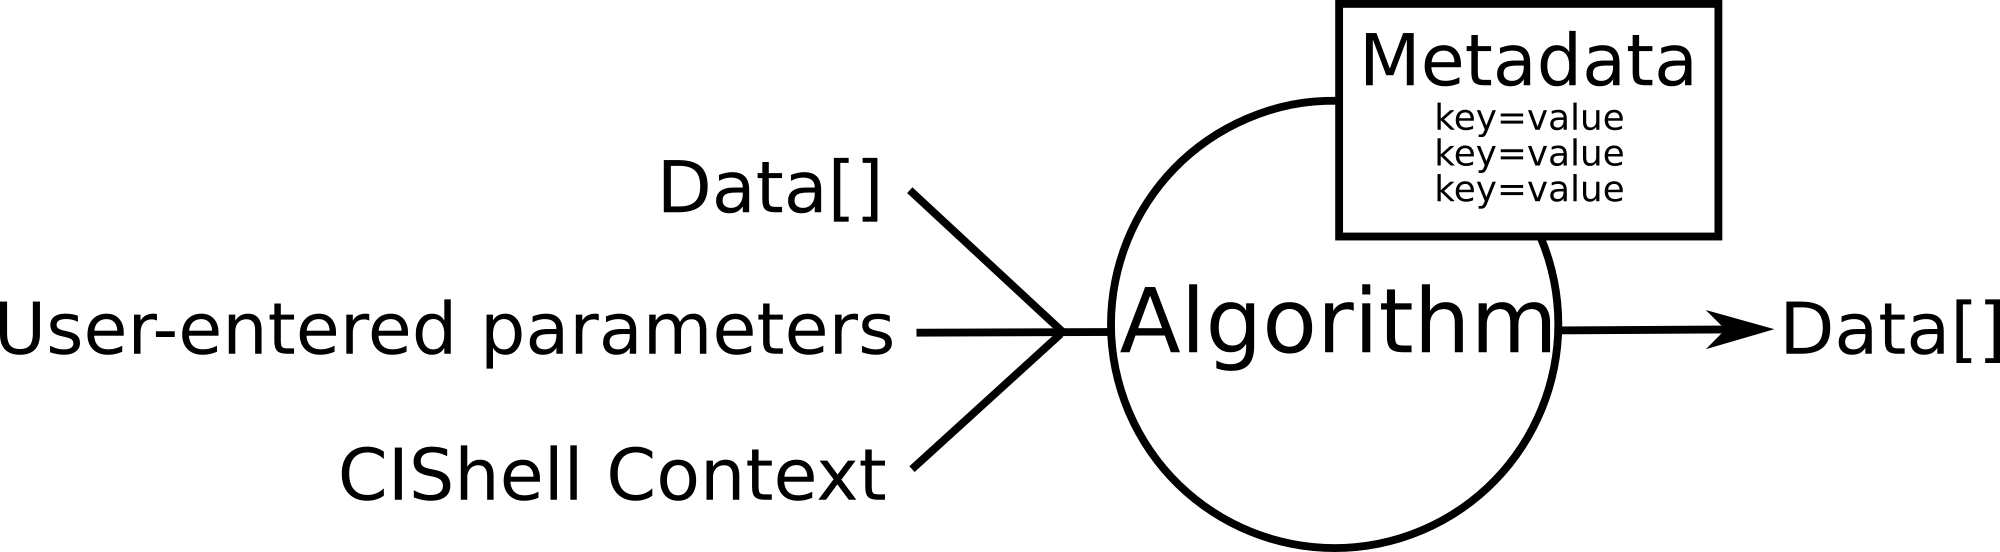
\includegraphics[width=50mm]{graphics/algorithmDefn.png} 
\end{center}
%\end{wrapfigure} 

Using CIShell, datasets and algorithms are bundled as CIShell-defined 
algorithms (see figure above). An algorithm is a black box that takes in 
zero or more datasets, some defined user parameters, and a so called CIShell 
Context. It then processes the inputs and returns an output in the form of zero 
or more datasets. The CIShell Context provides access to services offered by 
CIShell such as logging, preferences, GUI creation, and data conversion. The 
metadata dictionary associated with each algorithm can be used by applications 
to search with (see section 2.4). The metadata also comprises the author, 
citations, links to homepages, documentation, run-time complexity, etc. that 
ensures proper usage and citation.

To give an example, a modeling algorithm takes in no data, some user-entered 
parameters (e.g., the number of nodes to create a random graph) and returns a 
single dataset (e.g., a randomly generated graph). An analysis algorithm takes 
in some data and possibly some user-entered parameters, analyses the graph, 
then returns a new graph or simply prints out analysis results on the console. 
A visualization algorithm takes in some data, opens a new window visualizing 
the data, and typically returns no data. Each dataset is bundled as a ‘dataset 
provider’, i.e.,  an algorithm that takes in no data or parameters, but returns 
a dataset that is then loaded into the CIShell system.

\subsection{Algorithm \& Dataset Integration Templates}

To ease the integration of algorithms and datasets, wizard-driven templates are 
provided that acquire information from the algorithm writer and then generate 
the appropriate files and resources. Templates are available to integrate 
arbitrary file-based datasets, compiled executable code, Java libraries, and 
Java-based algorithms. In the case of the Java-based template, after running 
the wizard, only one method needs to be filled in. This is the execute method for 
the actual algorithm. Integration of executable code typically does not require 
writing even one line of new code.

\subsection{Algorithm \& Dataset Distribution}

Distribution of algorithms and datasets is made easy by using 
Eclipse \cite{eclipse} update sites and the NWB Community Wiki. Eclipse update 
sites allow an algorithm writer to package up their algorithms as features and 
place them on a webserver. Any algorithm writer can create his or her own 
private or public update site. Algorithm users can download any subset of 
datasets and algorithms from any number of update sites. He or she simply needs 
to select Help/Update from the menu and search for new features or updates of 
the currently installed features.

The NWB Community Wiki provides an easy interface for algorithm writers and data 
holders to post links to their algorithms and datasets, explain how to use 
them, and advertise their update sites (see section 4).

\subsection{Creating A Pool}

Algorithms defined in section 2.1 can be located and run by using a 
service registry that is provided by the underlying Open Services Gateway 
Initiative (OSGi) technology \cite{osgi}. This service registry defines a pool 
where services can be registered, searched for, and retrieved for use.
\begin{wrapfigure}{i}[-2mm]{22mm} 
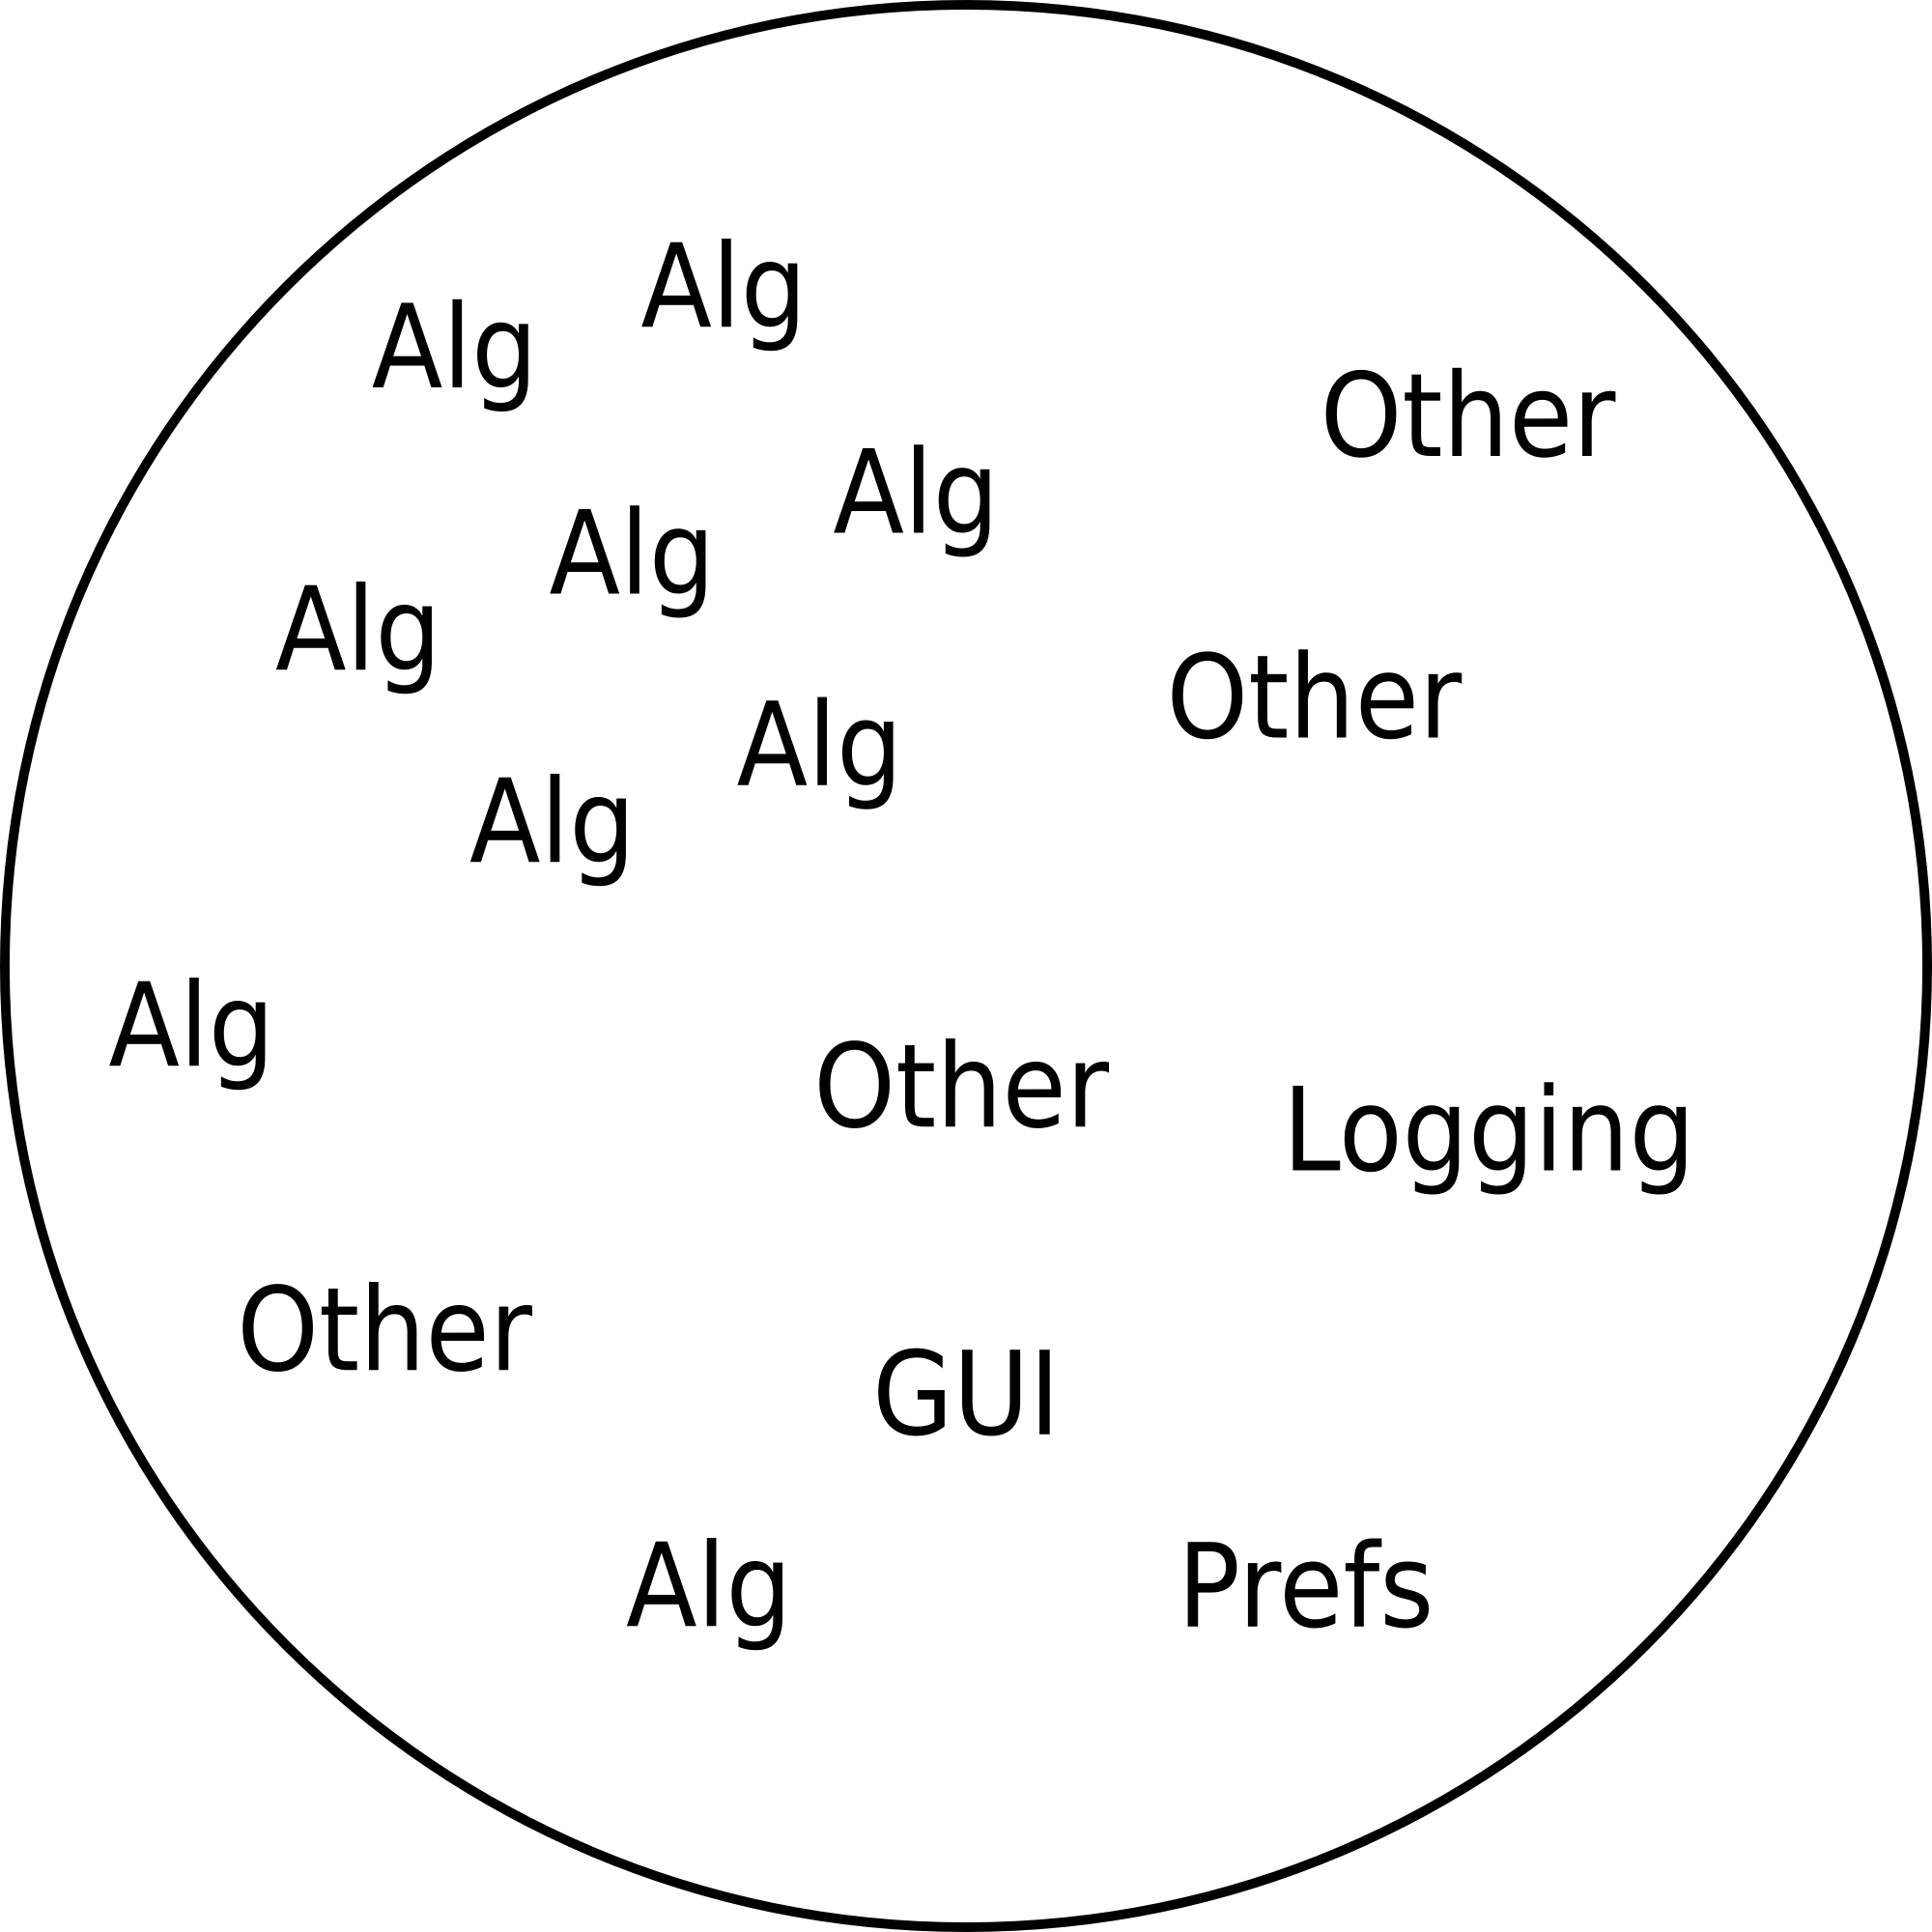
\includegraphics[width=22mm,height=22mm,clip=true]{graphics/algorithmPool.png} 
\end{wrapfigure} To be a service in OSGi, one must provide an interface, an 
implementation of the interface, and a dictionary of metadata about the 
service. For algorithms, the interface is AlgorithmFactory as defined by 
CIShell and the implementation and metadata as provided by the algorithm 
writer. All major components of CIShell are defined in terms of services 
available in the service registry.

Once the algorithms are in the service pool (see figure above), CIShell 
applications can easily search for algorithms based on their metadata. A 
querying mechanism can be used by applications to find subsets of algorithms 
like all algorithms that belong in the visualization menu, all converter 
algorithms, etc. This is important for automatically converting data (see 
section 2.7).

\subsection{Creating An Application}

Every application that uses CIShell technology utilizes the OSGi Service 
Registry to locate and run algorithms. For example, a graphical user interface 
(GUI) application searches for all algorithms that have a menu path and puts 
them in their appropriate GUI menu; a scripting layer allows scripts to gain 
access to the algorithms in the service registry, etc. That is, algorithms are 
independent of their usage.

\subsection{Connecting Pools \& Applications}

Our future work aims to create CIShell web services and to support the 
interlinkage of multiple algorithm pools and web services in a peer-to-peer 
fashion. This inter-pool communication mechanism (see figure below) will also 
support client-server applications in which computationally demanding 
algorithms are run on servers and multiple CIShell clients can connect to it to 
use datasets, algorithms, and computing power.

\begin{center}
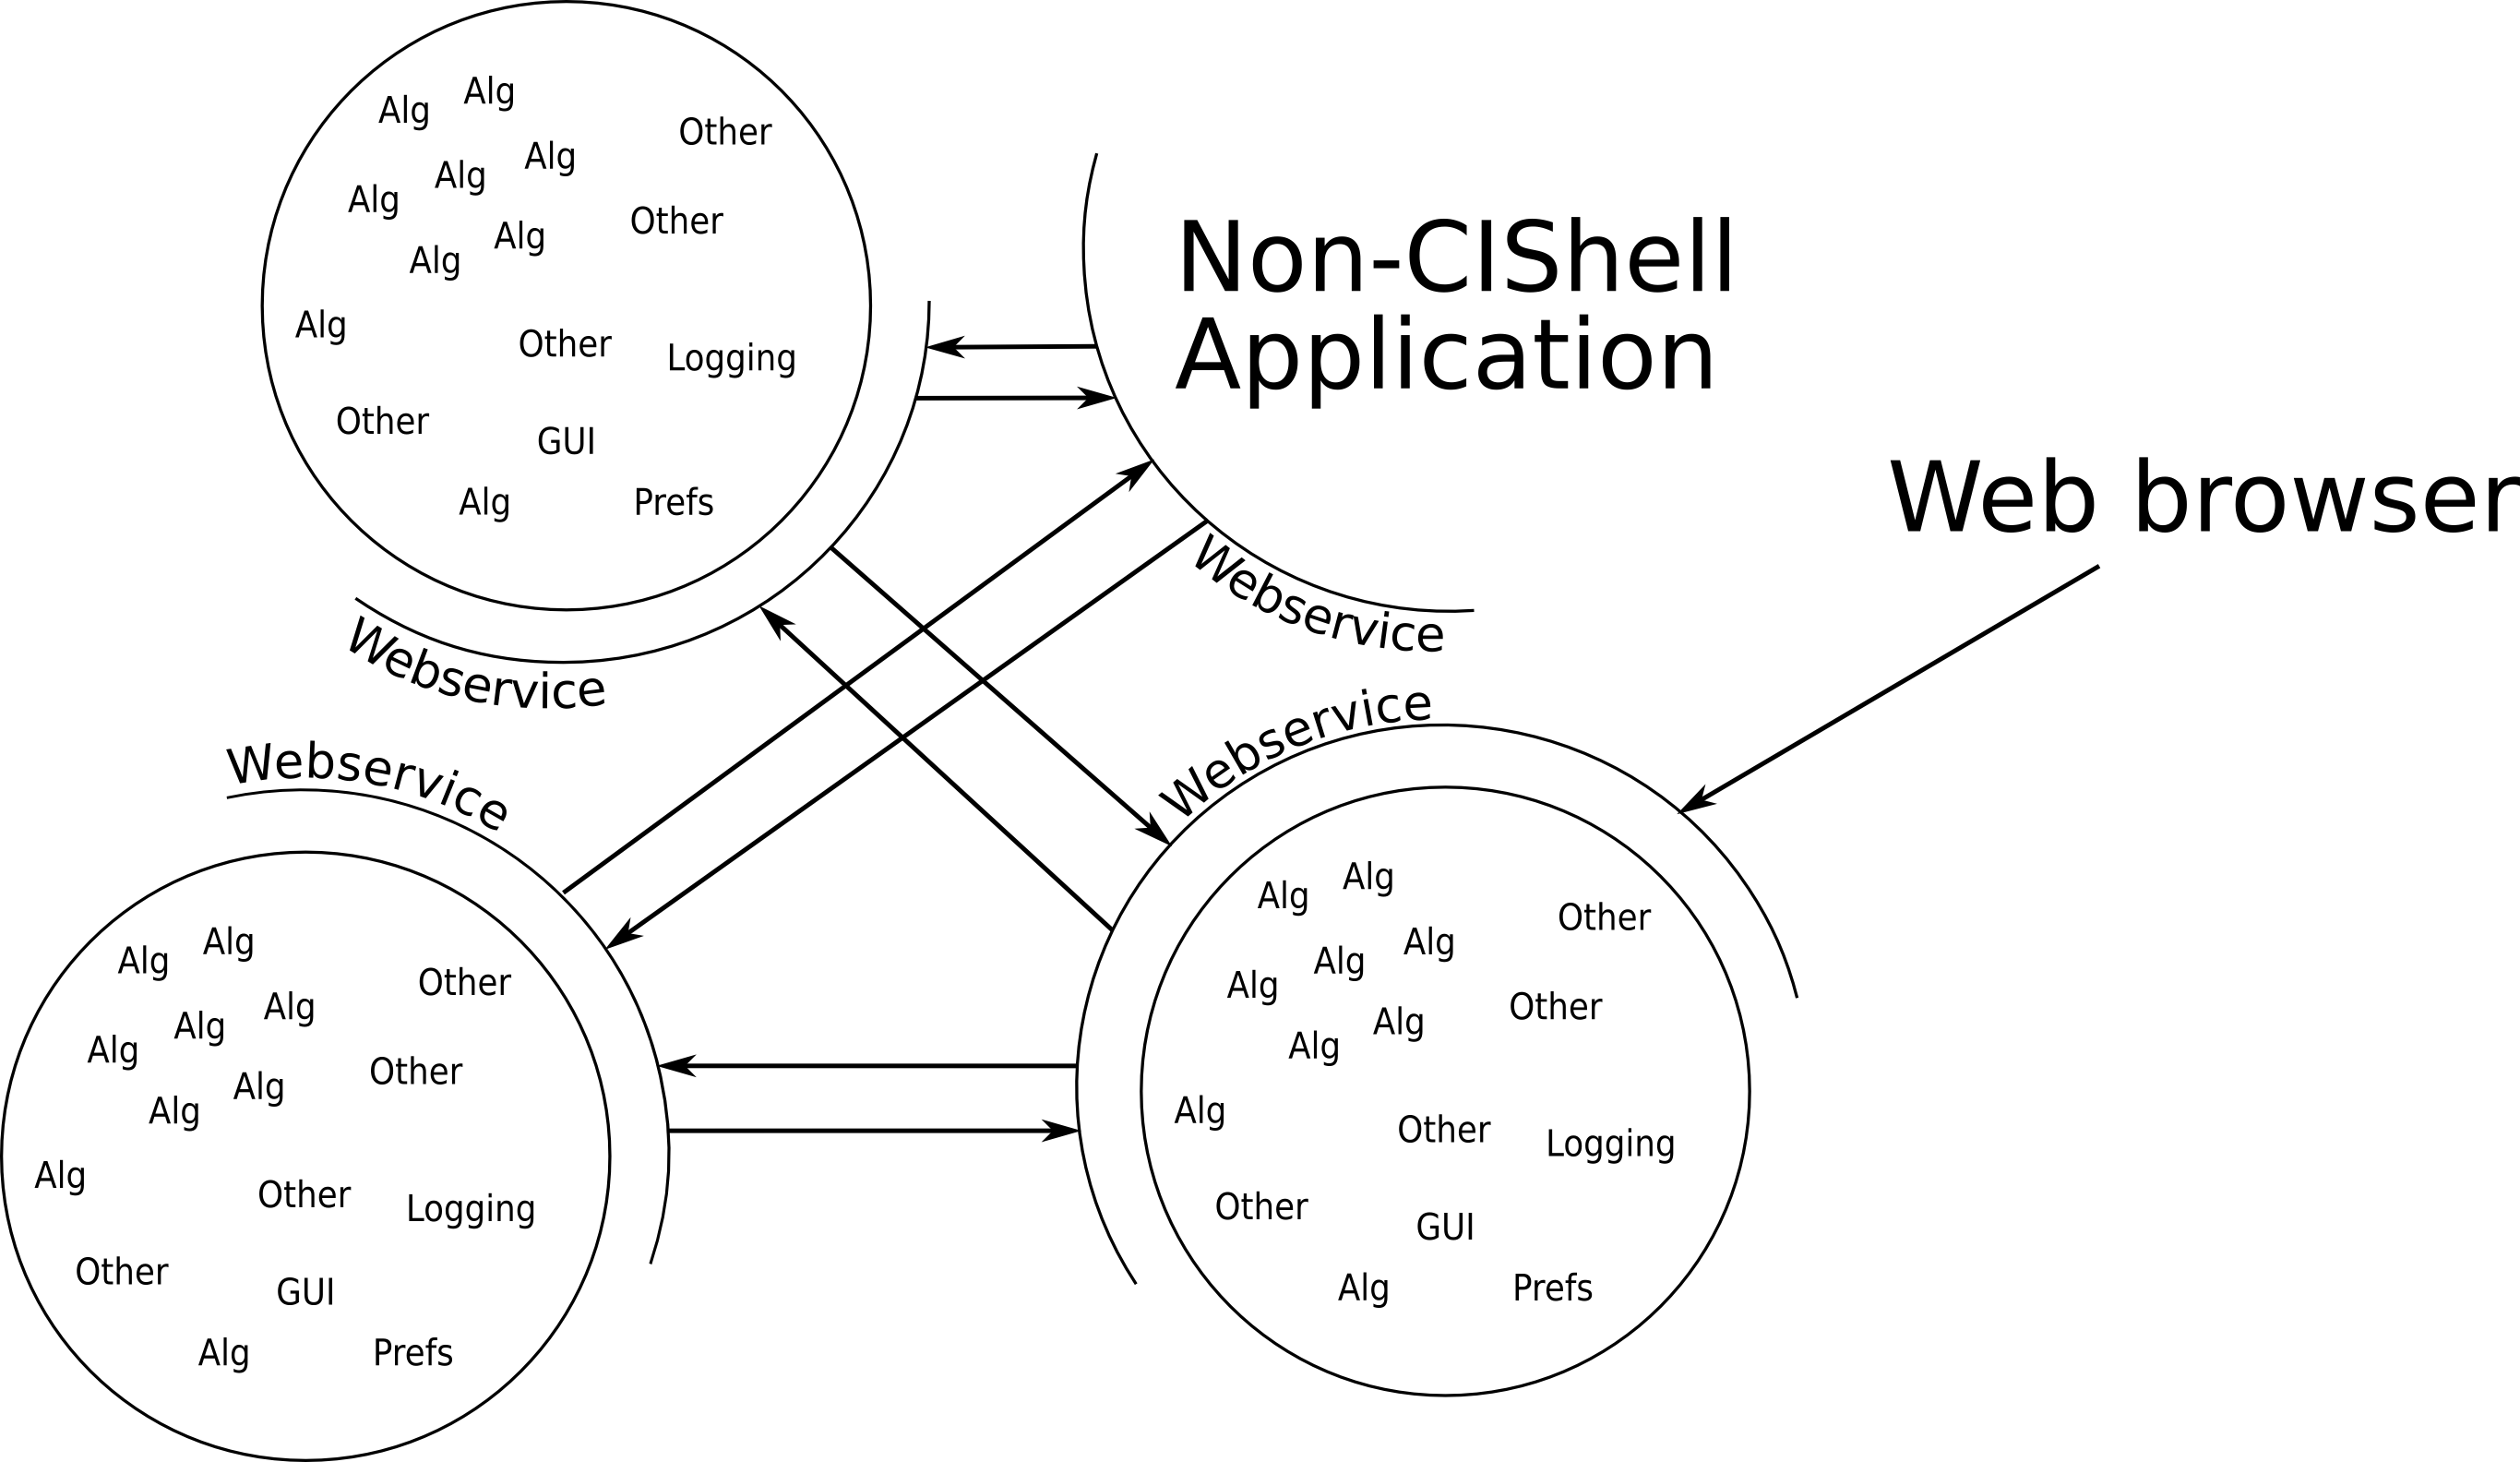
\includegraphics[width=70mm]{graphics/connectingPools.png}
\end{center}

\subsection{Automatic Data Conversion}

Algorithms and the service registry can be utilized to solve another problem 
that arises when dealing with many algorithms written by different people from 
different scientific communities: the multitude of existing file formats. The 
data conversion service offered by CIShell supports the seamless conversion of 
different file formats.

\begin{wrapfigure}{i}[-2mm]{40mm} 
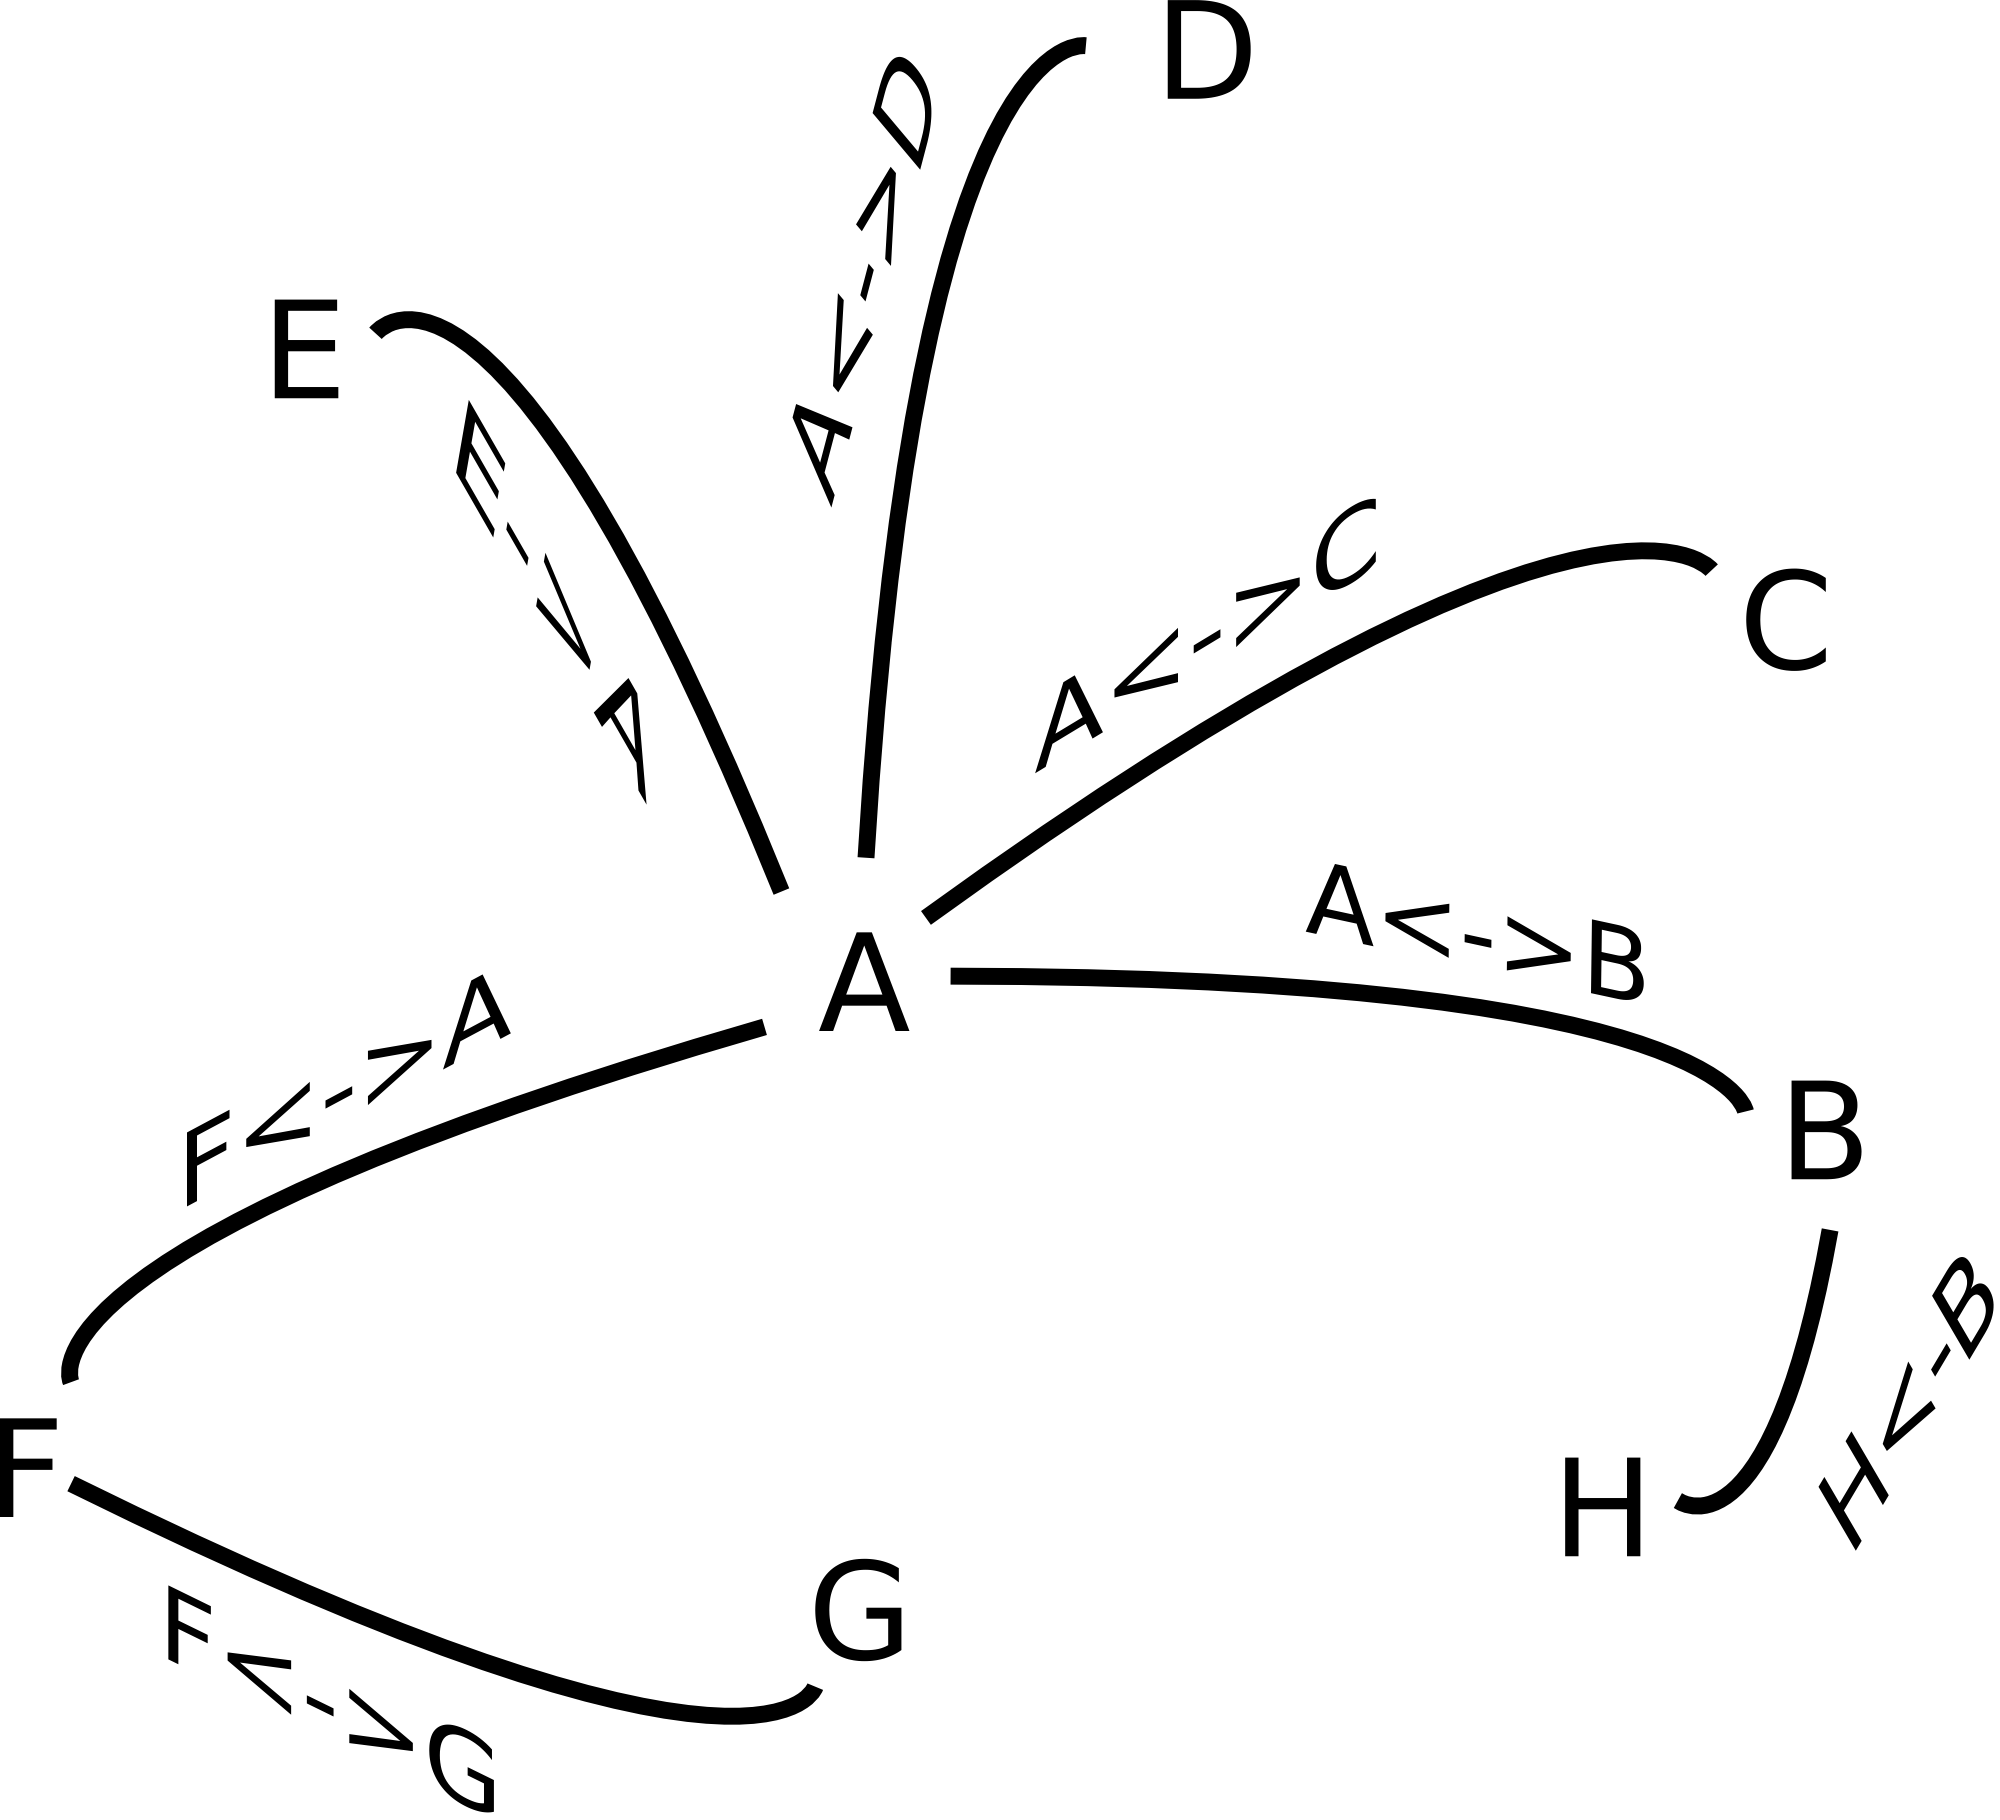
\includegraphics[width=40mm,clip=true]{graphics/conversionGraph.png}
\end{wrapfigure}

The service searches through the service registry for converter algorithms 
(type=conversion in the algorithm's metadata) and builds a directed graph based 
on them in which edges are converters and nodes are file formats (see figure to 
the right). Edges can be weighted according to the 'losslessness', 
'complexity', or other features as reported in a converters' metadata.

When asked to find a chain of converters from format A to format G, it searches 
the graph for the shortest (weighted) path and returns a valid chain of 
converters. The CIShell Reference GUI uses this data conversion service to 
identify those algorithms that can handle a selected dataset. Only applicable 
algorithms are selectable and only if the algorithm is selected will the data 
be converted into the appropriate format. Data format conversion happens 
invisibly to the user.

\subsection{Brandable CIShell Reference GUI}

The CIShell project includes a reference GUI that can be used directly or 
customized by application writers. The GUI (see figure below) is a menu-driven 
interface where all algorithms appears as menu items. Datasets can be loaded or 
simulated and are listed in the right-hand side data manager. When a user 
selects a dataset, the GUI determines if it can be used by any algorithms 
(either directly or through a series of converters). Only algorithms that can 
process the selected dataset are clickable, all others are grayed out. A 
console is provided to give information about the selected algorithms (authors, 
implementers, citations, etc.) and any output the algorithm logs when run. 

\begin{center}
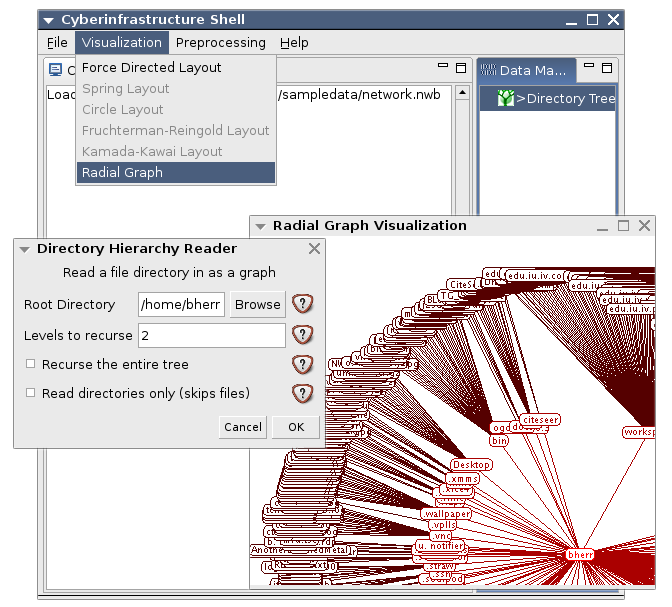
\includegraphics[width=2.24in]{graphics/cishell-using1.png}
\end{center}